
%
%	Sketches for Q12(b)(i)

%
%	The Region R
%
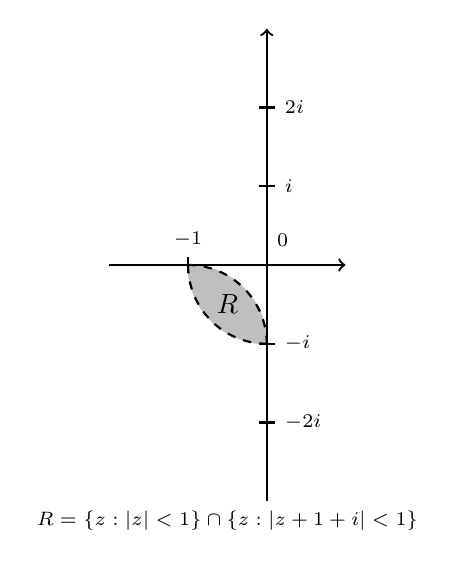
\begin{tikzpicture}
	% shading - must be drawn before the rest!
	\filldraw[color=lightgray] (-1,0) arc (0:90:-1) (0,-1) arc (0:90:1);
	\draw (-0.5,-0.5) node {$R$};
	% grid for draft only
	%%\draw [help lines] (-2,-3) grid (1,3);
	% legend
	\draw (-0.5,-3) node[below] {\scriptsize $R=\{z:|z|<1\} \cap \{z:|z+1+i|<1\}$};
	% the X-axis
	\draw[->,thick] (-2,0)--(1,0);
	\draw[thick] (-1,-0.1) -- (-1,0.1) node[above] {\scriptsize $-1$};
	\draw[thick] ( 0,-0.1) -- ( 0,0.1) node[above right] {\scriptsize $0$};
	% the Y-axis
	\draw[->,thick] (0,-3)--(0,3);
	\draw[thick] (-0.1,-1) -- (0.1,-1) node[right] {\scriptsize $-i$};
	\draw[thick] (-0.1,-2) -- (0.1,-2) node[right] {\scriptsize $-2i$};
	\draw[thick] (-0.1, 1) -- (0.1, 1) node[right] {\scriptsize $ i$};
	\draw[thick] (-0.1, 2) -- (0.1, 2) node[right] {\scriptsize $ 2i$};
	% inner circle border
	\draw[thick,style=dashed] (-1,0) arc (0:90:-1);
	% outer circle border
	\draw[thick,style=dashed] (0,-1) arc (0:90:1);
\end{tikzpicture}
%%\bigskip
%
%	The Region S
%
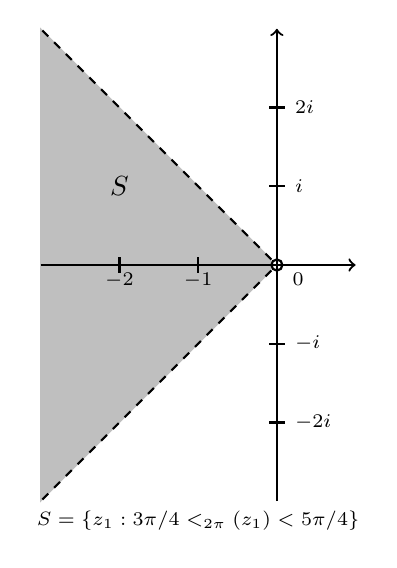
\begin{tikzpicture}
	% shading - must be drawn before the rest!
	\filldraw[color=lightgray] (-2pt,2pt) -- (-3,3) -- (-3,-3) -- (-2pt,-2pt);
	\draw (-2,1) node {$S$};
	% grid for draft only
	%%\draw [help lines] (-3,-3) grid (1,3);
	% legend
	\draw (-1,-3) node[below]
		{\scriptsize $S=\{z_1: 3\pi/4 < \Arg_{2\pi}(z_1) < 5\pi/4 \}$};
	% the X-axis
	\draw[->,thick] (-3,0)--(1,0);
	\draw[thick] (-2,-0.1) -- (-2,0.1) node[below=2pt] {\scriptsize $-2$};
	\draw[thick] (-1,-0.1) -- (-1,0.1) node[below=2pt] {\scriptsize $-1$};
	\draw[thick] ( 0,-0.1) -- ( 0,0.1) node[below right=2pt] {\scriptsize $0$};
	% the Y-axis
	\draw[->,thick] (0,-3)--(0,3);
	\draw[thick] (-0.1,-1) -- (0.1,-1) node[right] {\scriptsize $-i$};
	\draw[thick] (-0.1,-2) -- (0.1,-2) node[right] {\scriptsize $-2i$};
	\draw[thick] (-0.1, 1) -- (0.1, 1) node[right] {\scriptsize $ i$};
	\draw[thick] (-0.1, 2) -- (0.1, 2) node[right] {\scriptsize $ 2i$};
	% upper ray
	\draw[thick,style=dashed] (-2pt, 2pt) -- (-3,3);
	% lower ray
	\draw[thick,style=dashed] (-2pt,-2pt) -- (-3,-3);
	% exclude the origin
	\draw[thick] (0,0) circle(2pt);
\end{tikzpicture}

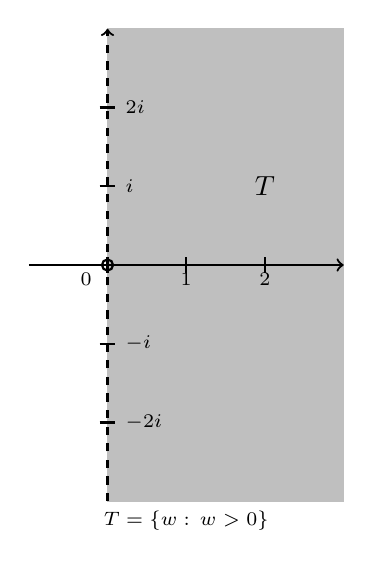
\begin{tikzpicture}
	% shading - must be drawn before the rest!
	\filldraw[color=lightgray] (0,3) -- (3,3) -- (3,-3) -- (0,-3) -- cycle;
	\draw (2,1) node {$T$};
	% grid for draft only
	%%\draw [help lines] (-1,-3) grid (3,3);
	% legend
	\draw (1,-3) node[below]
		{\scriptsize $T=\{ w: \RE\,w > 0 \} $};
	% the X-axis
	\draw[->,thick] (-1,0)--(3,0);
	\draw[thick] ( 2,-0.1) -- ( 2,0.1) node[below=2pt] {\scriptsize $ 2$};
	\draw[thick] ( 1,-0.1) -- ( 1,0.1) node[below=2pt] {\scriptsize $ 1$};
	\draw[thick] ( 0,-0.1) -- ( 0,0.1) node[below left=2pt] {\scriptsize $0$};
	% the Y-axis
	\draw[->,thick,style=dashed] (0,-3)--(0,3);
	\draw[thick] (-0.1,-1) -- (0.1,-1) node[right] {\scriptsize $-i$};
	\draw[thick] (-0.1,-2) -- (0.1,-2) node[right] {\scriptsize $-2i$};
	\draw[thick] (-0.1, 1) -- (0.1, 1) node[right] {\scriptsize $ i$};
	\draw[thick] (-0.1, 2) -- (0.1, 2) node[right] {\scriptsize $ 2i$};
	% exclude the origin
	\draw[thick] (0,0) circle(2pt);
\end{tikzpicture}
